%\documentclass{article}
\documentclass[10pt,a4paper]{report}
\usepackage{amsmath}
\usepackage{amssymb}
\usepackage{amssymb}
\usepackage{setspace}
\usepackage{tasks}
\usepackage{graphicx}
\usepackage{float}
\usepackage{listings}

%\documentclass[10pt,a4paper]{report}
%\usepackage[latin1]{inputenc}
\usepackage[utf8]{inputenc}
\usepackage{amsfonts}
\usepackage{multicol}
\usepackage{multicol}
\usepackage{tabularx}
\usepackage{tikz}
\usetikzlibrary{arrows,shapes,automata,petri,positioning,calc}
\usepackage{hyperref}
\usepackage{tikz}
\usetikzlibrary{matrix,calc}
\usepackage[margin=0.5in]{geometry}
% ---- power functions -----% 
\newcommand{\myvec}[1]{\ensuremath{\begin{pmatrix}#1\end{pmatrix}}}
\let\vec\mathbf

%\providecommand{\norm}[1]{\left\lVert#1\right\rVert}
%\providecommand{\abs}[1]{\left\vert#1\right\vert}
%\let\vec\mathbf

\newcommand{\mydet}[1]{\ensuremath{\begin{vmatrix}#1\end{vmatrix}}}
\providecommand{\brak}[1]{\ensuremath{\left(#1\right)}}
\providecommand{\lbrak}[1]{\ensuremath{\left(#1\right.}}
\providecommand{\rbrak}[1]{\ensuremath{\left.#1\right)}}
\providecommand{\sbrak}[1]{\ensuremath{{}\left[#1\right]}}
\providecommand{\norm}[1]{\left\lVert#1\right\rVert}
\providecommand{\abs}[1]{\left\vert#1\right\vert}
\let\vec\mathbf
%\newcommand{\norm}[1]{\lVert#1\rVert}
\renewcommand{\vec}[1]{\textbf{#1}}
\begin{document}
\onehalfspacing
\begin{center}
	\section*{\textbf{Class 11}}
	\subsection*{Chapter 10 - STRAIGHT LINES}
\end{center}
The following problem is question 11 from exercise 10.4
\begin{enumerate}
    \item Find the equation of the lines through the point (3, 2) which make an angle of 45\textdegree \hspace{0.1cm} with the line x – 2y = 3.
\end{enumerate}
\textbf{Solution:}\\
The given line parameters are
\begin{align}
   \vec{n}=\myvec{1\\-2},c=-5
\end{align}
yielding
\begin{align}
\vec{m}=\myvec{1\\m}\\
\vec{m}=\myvec{2\\1}
\end{align}
where  $m$ is defined to be the slope of the line. If the angle between the lines be $\theta$,\\

\begin{align}
\cos \theta = \frac{m_1^\top m_2}{\norm{m_1}\norm{m_2}}\\
given\hspace{0.3cm}  \theta = 45^\circ\\
\implies cos45^\circ =  \frac{m_1^\top m_2}{\norm{m_1}\norm{m_2}}\\
\implies \frac{1}{\sqrt{2}} = \frac{\myvec{2 & 1} \myvec{1\\m}}{\norm{\myvec{2\\1}}\norm{\myvec{1\\m}}}\\
\\
\implies \frac{1}{\sqrt{2}}=\frac{2+m}{\sqrt{2^2 + 1}\sqrt{m^2 + 1}}\\
\\
\implies \frac{1}{2}=\frac{m^2 + 4m +4}{5m^2 +5}\\
\text{or, } 3m^2 - 8m -3 = 0
\end{align}
yielding
\begin{align}
m= - \frac{1}{3}, 
 3
\end{align} 
 A line passes through (x, y) and (h, k). If slope of the line is m then
\begin{align}
(k-y) = m(h-x)\\
\text{when, } m=3 \hspace{0.3cm} and \hspace{0.3cm} (h,k)=(3,2)\\
    2-y=3(3-x)\\
     y-2=3x-9\\
    3x-y=7\\
    \implies (3 \hspace{0.3cm} -1)x=7
\end{align}
And, when $m=-\frac{1}{3}$,\\
The equation of the line passing through (3,2) and having a slope of $-\frac{1}{3}$ is
\begin{align}
    2-y=-\frac{1}{3}(3-x)\\
    3y-6=-x+3\\
    x+3y=9\\
    \implies (1 \hspace{0.4cm} 3)x=9
\end{align}
Therefore, the equations of the lines are 
\begin{align}
 (3 \hspace{0.2cm} -1)x=7    \hspace{0.3cm}and\hspace{0.3cm} (1 \hspace{0.4cm} 3)x=9 .
\end{align}
\begin{figure}[H]
\centering
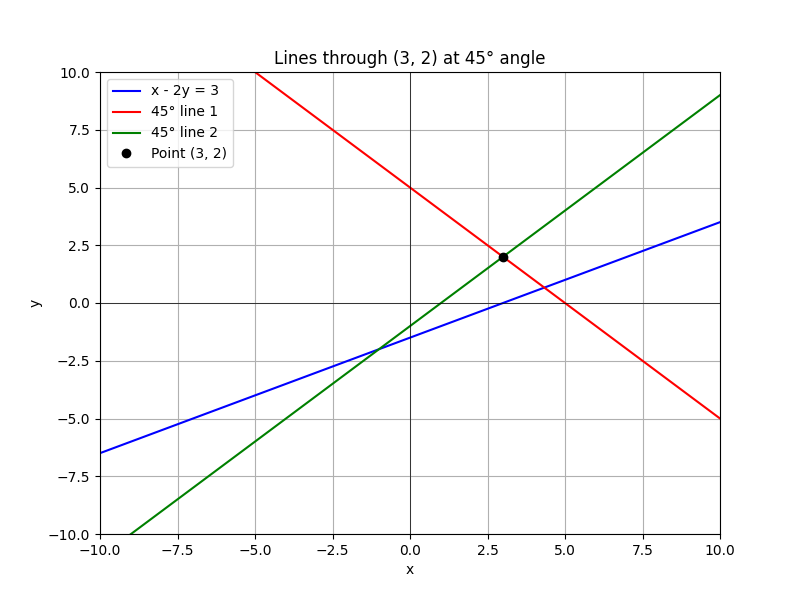
\includegraphics[width=0.7\textwidth]{figs/line.jpg}
\caption{STRAIGHT LINES}
\label{fig:line.jpg}
\end{figure}




\end{document}s
